% Options for packages loaded elsewhere
\PassOptionsToPackage{unicode}{hyperref}
\PassOptionsToPackage{hyphens}{url}
%
\documentclass[
  a4paper,
]{article}
\usepackage{amsmath,amssymb}
\usepackage{setspace}
\usepackage{iftex}
\ifPDFTeX
  \usepackage[T1]{fontenc}
  \usepackage[utf8]{inputenc}
  \usepackage{textcomp} % provide euro and other symbols
\else % if luatex or xetex
  \usepackage{unicode-math} % this also loads fontspec
  \defaultfontfeatures{Scale=MatchLowercase}
  \defaultfontfeatures[\rmfamily]{Ligatures=TeX,Scale=1}
\fi
\usepackage{lmodern}
\ifPDFTeX\else
  % xetex/luatex font selection
\fi
% Use upquote if available, for straight quotes in verbatim environments
\IfFileExists{upquote.sty}{\usepackage{upquote}}{}
\IfFileExists{microtype.sty}{% use microtype if available
  \usepackage[]{microtype}
  \UseMicrotypeSet[protrusion]{basicmath} % disable protrusion for tt fonts
}{}
\makeatletter
\@ifundefined{KOMAClassName}{% if non-KOMA class
  \IfFileExists{parskip.sty}{%
    \usepackage{parskip}
  }{% else
    \setlength{\parindent}{0pt}
    \setlength{\parskip}{6pt plus 2pt minus 1pt}}
}{% if KOMA class
  \KOMAoptions{parskip=half}}
\makeatother
\usepackage{xcolor}
\usepackage[margin=1in]{geometry}
\usepackage{graphicx}
\makeatletter
\def\maxwidth{\ifdim\Gin@nat@width>\linewidth\linewidth\else\Gin@nat@width\fi}
\def\maxheight{\ifdim\Gin@nat@height>\textheight\textheight\else\Gin@nat@height\fi}
\makeatother
% Scale images if necessary, so that they will not overflow the page
% margins by default, and it is still possible to overwrite the defaults
% using explicit options in \includegraphics[width, height, ...]{}
\setkeys{Gin}{width=\maxwidth,height=\maxheight,keepaspectratio}
% Set default figure placement to htbp
\makeatletter
\def\fps@figure{htbp}
\makeatother
\setlength{\emergencystretch}{3em} % prevent overfull lines
\providecommand{\tightlist}{%
  \setlength{\itemsep}{0pt}\setlength{\parskip}{0pt}}
\setcounter{secnumdepth}{-\maxdimen} % remove section numbering
\ifLuaTeX
\usepackage[bidi=basic]{babel}
\else
\usepackage[bidi=default]{babel}
\fi
\babelprovide[main,import]{catalan}
% get rid of language-specific shorthands (see #6817):
\let\LanguageShortHands\languageshorthands
\def\languageshorthands#1{}
\ifLuaTeX
  \usepackage{selnolig}  % disable illegal ligatures
\fi
\usepackage{bookmark}
\IfFileExists{xurl.sty}{\usepackage{xurl}}{} % add URL line breaks if available
\urlstyle{same}
\hypersetup{
  pdfauthor={@tofermos 2024},
  pdflang={ca-ES},
  hidelinks,
  pdfcreator={LaTeX via pandoc}}

\title{Instal·lació de Windows 11 en VirtualBox}
\author{@tofermos 2024}
\date{}

\begin{document}
\maketitle

{
\setcounter{tocdepth}{2}
\tableofcontents
}
\setstretch{1.5}
\newpage

\renewcommand\tablename{Tabla}

\section{Resum}\label{resum}

El següent document només conté alguns recordatoris i consells sobre la
instal·lació d'un Windows 11 en una VirtualBox.

\section{1 Recursos}\label{recursos}

\section{2 Consideracions en la instal·Lació de
VirtualBox}\label{consideracions-en-la-installaciuxf3-de-virtualbox}

En crear i configurar la màquina, hem de revisar el l'ordre d'arrencada
de la màquina.

\begin{itemize}
\tightlist
\item
  Convé desmarcar el Disquette.
\item
  Seleccionar TPM (Versió 2.0)
\item
  Activar la EFI
\end{itemize}

El TPM (Mòdul de Plataforma Segura) és un xip de seguretat que
emmagatzema claus criptogràfiques i dades sensibles en un ordinador.
Ajuda a protegir el sistema operatiu i a evitar accessos no autoritzats,
especialment en funcions com el xifratge de disc o l'autenticació
segura.

\includegraphics[width=0.7\textwidth,height=\textheight]{png/configuracióMV.png}

Vegem les característiques de HW necessari.

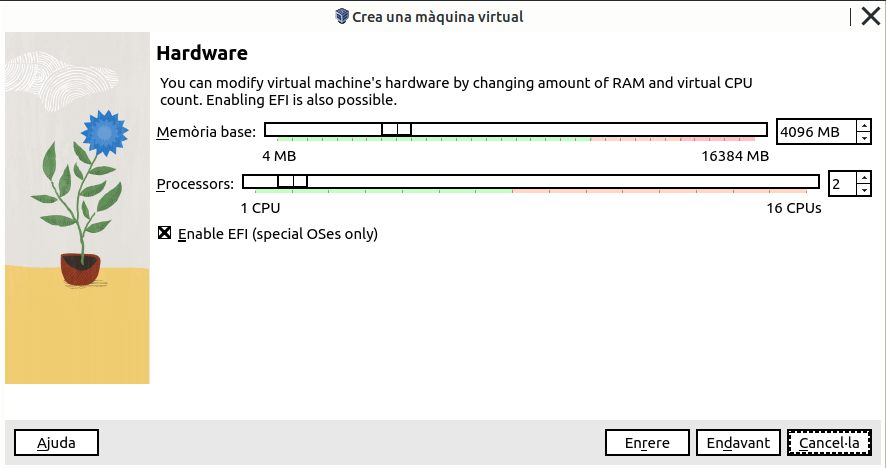
\includegraphics[width=0.7\textwidth,height=\textheight]{png/Hardware.png}

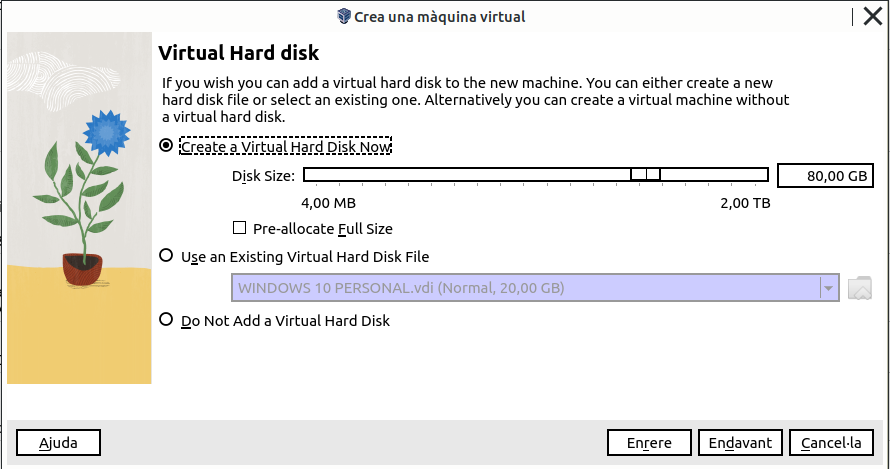
\includegraphics[width=0.7\textwidth,height=\textheight]{png/Hardware2.png}

En crear la màquina virtual hem d'especificar en quin disc volem que
s'instal·le.

Per poder instal·lar en un \textbf{DISC EXTRAÏBLE} només hem
d'especificar la carpeta destí en l'aparatat \textbf{FOLDER}

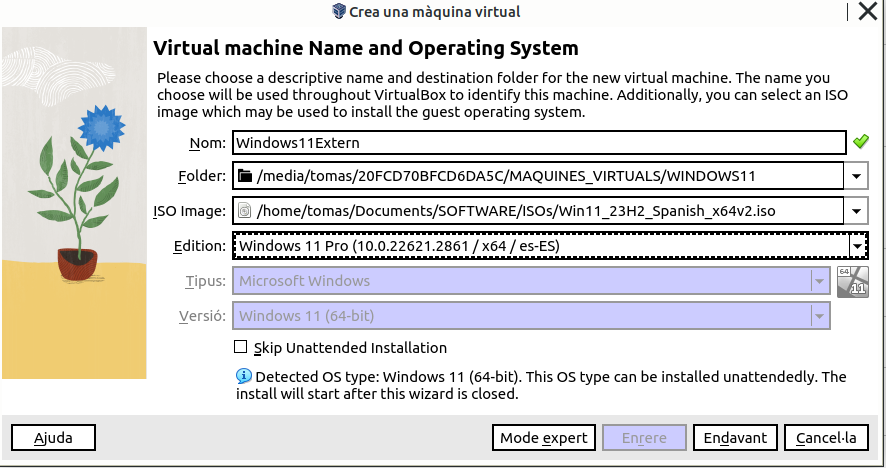
\includegraphics[width=0.7\textwidth,height=\textheight]{png/SeleccioCarpetaDesti.png}

\section{3 Error habitual\ldots{}}\label{error-habitual}

Un error habitual és el següent\ldots{}

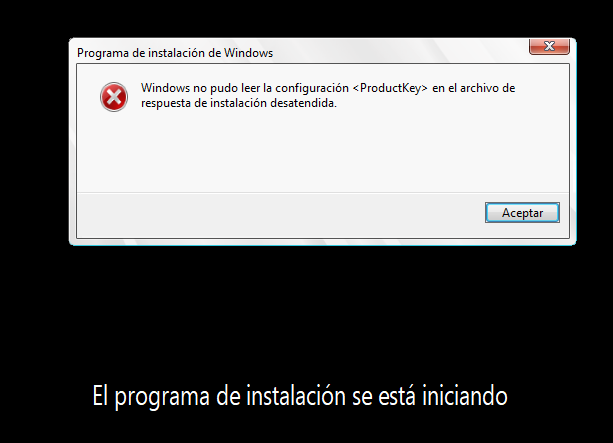
\includegraphics[width=0.7\textwidth,height=\textheight]{png/errorInstalacio.png}

\textbf{La solució} consisteix en elimimar un fitxer de la carpeta de
les instatànies.

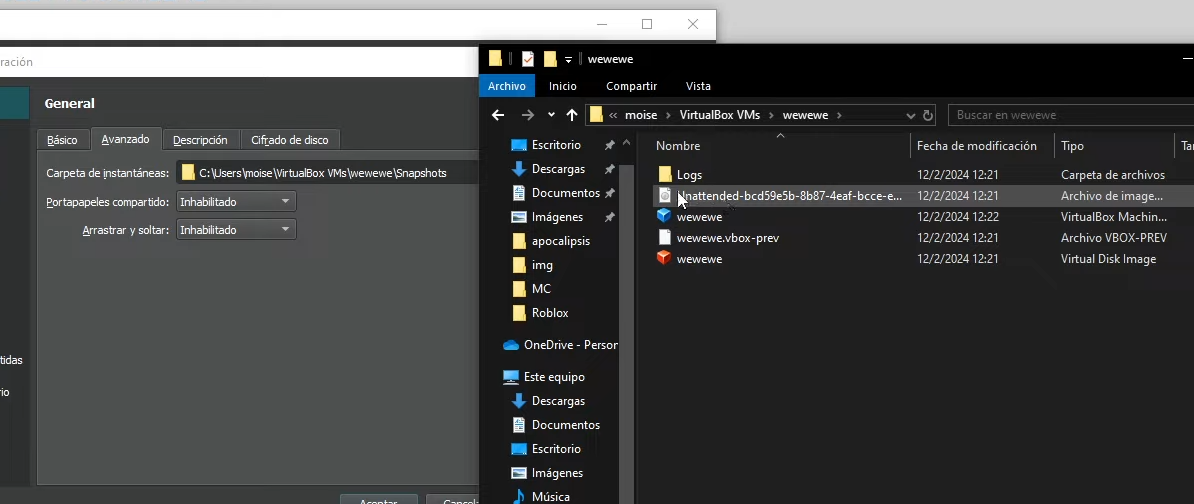
\includegraphics[width=0.9\textwidth,height=\textheight]{png/unattendedEliminar.png}

\end{document}
